\section{Dealing with Modeloutput}

\subsection{EURO-CORDEX-Data}
A lot of information is stored at the homepage:\\
e.g. User-Guide, Errata-page at \url{http://www.euro-cordex.net}

\subsection{Remapping tools}
\url{https://wiki.gerics.de/euro-cordex/RemappingMethods}

\subsection{Plotting tool}
\begin{itemize}
 \item For plotting results: e.g. PyPlotTools, documentation is in the ArcDoc
 
 \item Monitoring a REMO-RUN: e.g. Clidas, documentation is in the ArcDoc
\end{itemize}
\subsection{Download multiple files from a web page}

example page: \url{http://exporter.nsc.liu.se/8d168f8152704e67968ea28b19ab712e/ICHEC-EC-EARTH/day/}
{\small 
\begin{verbatim}
wget -r -nd -np -e robots=off -A.nc 
    http://exporter.nsc.liu.se/8d168f8152704e67968ea28b19ab712e/ICHEC-EC-EARTH/day/
\end{verbatim}}

explanation:
\begin{itemize}
\item[-r] signifies that wget should recursively download data in any subdirectories it finds.
\item[-l1] sets the maximum recursion to 1 level of subfolders.
\item[-nd] copies all matching files to current directory. If two files have identical names it appends an extension.
\item[-nc] does not download a file if it already exists.
\item[-np] prevents files from parent directories from being downloaded.
\item[-e robots=off] tells wget to ignore the robots.txt file. If this command is left out, the robots.txt file tells wget that it does not like web crawlers and this will prevent wget from working.
\item[-A.nc] restricts downloading to the specified file types (with .nc suffix in this case)
\end{itemize}

\subsection{Comparing REMO output to Observations}

\subsubsection{Observations have a different grid resolution than REMO output}

\textbf{Important}: You can only remap to the coarser grid, otherwise you recieve empty grid boxes!

\textbf{Attention}: If grids are very similar, you can also recieve empty gridboxes by using cdo remap.
\begin{enumerate}
\item Version 1: remap remo data to the grid of the observations (pay attention to different remapping
methods for each variable and remember to use height correction for temperature,
also see scripts in clidas and wiki-Page remapping tools.

\item Version 2: If you want to compare area means, you can also remap your remo-mask with \texttt{remapnn} to the grid of the observations.

\item Version 3: If you want to compare a single location to REMO output, consider the method of Standort Factsheets 
\end{enumerate}

\textbf{Height correction} Comparing temperature values of two different kind of files, you need to apply a height correction. 
Differences of the two orographie files $\Delta height times 0,0065 K$.

\subsubsection{Area mean of small catchments}

e.g. For the Hamburg port area, the value is weighted (e.g. precipitation) of each grid cell with the fraction of that grid cell which covered the port area. 

For this, Thomas Raub calculated the fraction of each grid cell which covered the catchment, see figure attached. 
\url{https://git.gerics.de/GERICS_products/HPA-Factsheet}

\begin{figure} [h!tb]
\begin{center}
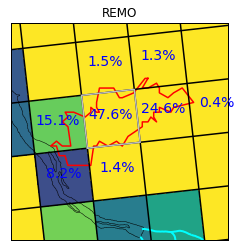
\includegraphics[width=5cm, natwidth=200, natheight=195]{./fig/krueckau_weights_REMOdetailliert.png} \\
\caption{Method of weighted mean for small areas}
\end{center}
\end{figure}
\figure

%\subsubsection{Compare station data to REMO output}
%has not been tested:
%\subsubsection{Compare station data to REMO output}

\bf{1.} Make unstructured grid  - for 22 stations NUM=22:\\
xvals and yvals are of the station:\\
\#
\# gridID 2
\#
gridtype  = unstructured
gridsize  = 22
xname     = lon
xunits    = degrees\_east
yname     = lat
yunits    = degrees\_north
nvertex   = 0
xvals     = 24.21570 27.020736 24.13184 26.37311 23.191068 26.430780 23.5750679 22.352339 21.011436  23.064745
            21.112153 25.2016275 27.165034 24.065786 25.221784 22.301310 25.074154 24.244387 22.330275 21.321429
            25.5505675 25.542023
yvals     = 57.520400 57.262248 56.22451 55.521139 56.371165 57.075598 56.3324954 57.444939 56.283135
	    57.195964 56.531819 57.1856161 56.324096 56.570216 57.531171 56.403146 56.383328 57.18022 
            57.110021 57.234402 56.3111952 57.080628


\bf{2.} make wights for REMO grid 

cdo genbil,n32 REMO\_file remoweights.nc

\bf{3.} interpolation

cdo -r -remap,unstructured\_grid,remoweights.nc -smooth9  REMO\_file  22\_stations\_file

\bf{4.} extract stations
location = 1…22

cdo selindexbox,\${location},\${location},1,1 -setgrid,r\${NUM}x1 REMO\_file  22\_stations\_file REMO\_Station\_1

cdo outputts REMO\_Station\_1> REMO_Station\_1txt






\subsection{Useful \texttt{cdo} hints}
\url{https://code.mpimet.mpg.de/projects/cdo/}

\subsubsection{\texttt{cdo ensmean}}
\texttt{cdo ensmean} only works if all rcm simulations are on an identical grid.
Check grid with \texttt{cdo griddes}

\subsubsection{\texttt{selindexbox} and keep rotated grid by using \texttt{cdo}}
If you use \texttt{cdo} version 1.9.5 you can select rlon, rlat and you can even select a subgrid with \texttt{selindexbox} and still preserve rlon/rlat
(this was not the case in earlierer cdo-versions, they would get grid of the rlon/rlat grid information and would only keep lat/lon grid)

\subsubsection{Change rotated grid rlon/rlat to lon/lat}
If you want to change the rlon/rlat of a remo-file to lat/lon grid, you can use \texttt{cdo setgridtype curvilinear}

\subsection{Useful \texttt{netcdf file} hints}

\subsubsection{Delete history}
If you like to give away a data file or publish it in a publication and do not want to publish its history. 
You can delete the whole history:
ncatted -h -a history,global,d,, old-file.nc new-file.nc

\subsubsection{Change unit}
If you changed the unit of the data file from e.g. Celcius to Kelvin, you should also change the unit in the header
have a look first how your variable is called  (ncdump -h) 
e.g. Variable: tg
ncatted -O -a units,tg,o,c,"Kelvin" -h file.nc

